\documentclass{article}

% if you need to pass options to natbib, use, e.g.:
%     \PassOptionsToPackage{numbers, compress}{natbib}
% before loading neurips_2018

% ready for submission
% \usepackage{neurips_2018}

% to compile a preprint version, e.g., for submission to arXiv, add add the
% [preprint] option:
 % \usepackage[preprint]{neurips_2018}

% to compile a camera-ready version, add the [final] option, e.g.:
 \usepackage[final]{neurips_2019}
% to avoid loading the natbib package, add option nonatbib:
%     \usepackage[nonatbib]{neurips_2018}
\usepackage{graphicx}
\usepackage[utf8]{inputenc} % allow utf-8 input
\usepackage[T1]{fontenc}    % use 8-bit T1 fonts
\usepackage{hyperref}       % hyperlinks
\usepackage{url}            % simple URL typesetting
\usepackage{booktabs}       % professional-quality tables
\usepackage{amsfonts}       % blackboard math symbols
\usepackage{nicefrac}       % compact symbols for 1/2, etc.
\usepackage{microtype}      % microtypography
\usepackage{amsmath}
\usepackage{bm}
\usepackage[english]{babel}
\usepackage{algorithm}
\usepackage{algorithmic}
\usepackage{appendix}
\newtheorem{theorem}{Theorem}
\newtheorem{lemma}{Lemma}
\newtheorem{proof}{Proof}
\input macros.tex
\title{Multi-way block localization vis sparse tensor clustering}

% The \author macro works with any number of authors. There are two commands
% used to separate the names and addresses of multiple authors: \And and \AND.
%
% Using \And between authors leaves it to LaTeX to determine where to break the
% lines. Using \AND forces a line break at that point. So, if LaTeX puts 3 of 4
% authors names on the first line, and the last on the second line, try using
% \AND instead of \And before the third author name.

\author{%
Yuchen Zeng \\
 University of Wisconsin -- Madison\\
 \texttt{yzeng58@wisc.edu} \\
\And
Miaoyan Wang \\
 University of Wisconsin -- Madison\\
\texttt{miaoyan.wang@wisc.edu} \\
%Madison, WI 53703 \\
% Affiliation \\
  % Address \\
  % \texttt{email} \\
  % \AND
  % Coauthor \\
  % Affiliation \\
  % Address \\
  % \texttt{email} \\
  % \And
  % Coauthor \\
  % Affiliation \\
  % Address \\
  % \texttt{email} \\
  % \And
  % Coauthor \\
  % Affiliation \\
  % Address \\
  % \texttt{email} \\
}

\begin{document}
% \nipsfinalcopy is no longer used

\maketitle

\begin{abstract}
 We consider the task of simultaneously clustering each mode of a large noisy tensor. We assume that the tensor elements are distributed with a block-specific mean and propose a least-square estimation for multi-way clustering. An $\ell_1$ penalty is applied to the block-means in order to select and identify important blocks. We show that our method is applicable to large tensors with a wide range of multi-way cluster structure, including a single block, multiple blocks, checkerboard clusters, 1-way or lower-way blocks. Our proposal amounts to a sparse, multi-way version of $k$-mean clustering, and a relaxation of our proposal yields the tensor Tucker decomposition. The performance of our proposals are demonstrated in simulations and on... 
\end{abstract}

\section{Introduction}
In recent years, much interest has centered around the unsupervised analysis of high-dimensional high-order tensor data. ....


Here is an example of tensor clustering by using our proposed method.
\begin{figure}[!h]
	\centering
	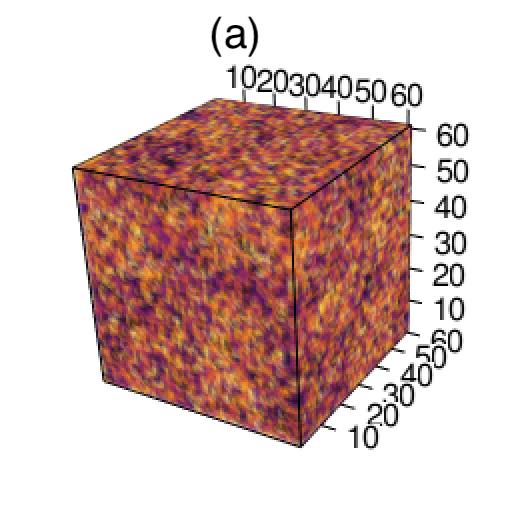
\includegraphics[scale=0.35]{figures/figure1/input.png}
	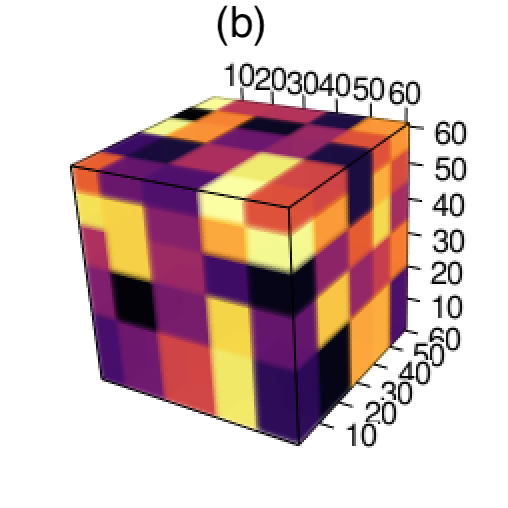
\includegraphics[scale=0.35]{figures/figure1/truth.png}
	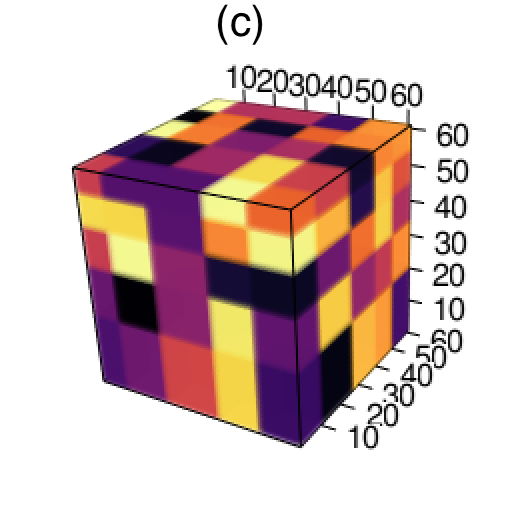
\includegraphics[scale=0.35]{figures/figure1/output.png}
	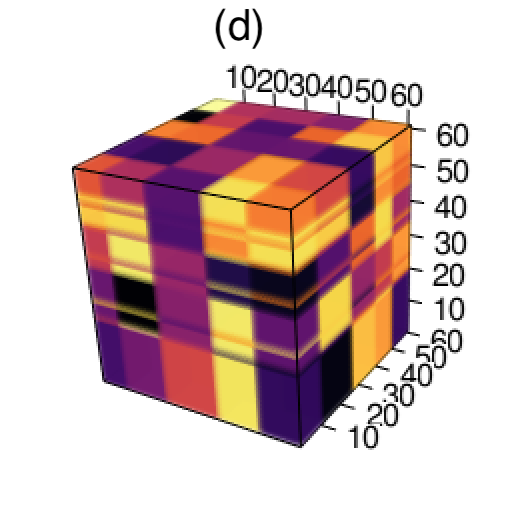
\includegraphics[scale=0.35]{figures/figure1/k_means.png}
	\caption{(a): a 60*60*60 tensor with 5 clusters in each mode; (b): true underlying mean signal within each cluster; (c): mean signal estimated by our proposed approach with true number of clusters: 5, 5, 5; (d): mean signal estimated by k-means clustering on each mode with true number of clusters:5 , 5, 5.}
	\label{fig1}
\end{figure}

\begin{figure}
	\centering
	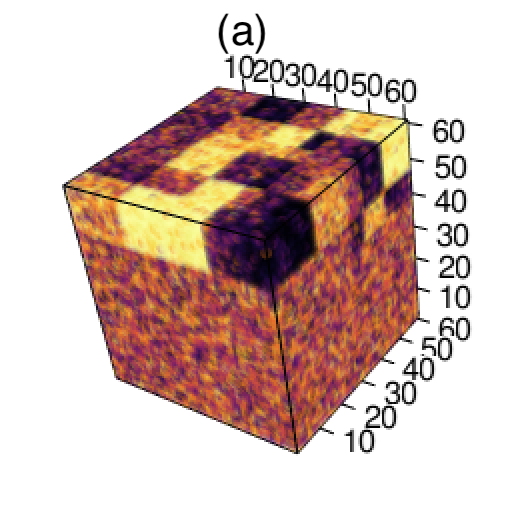
\includegraphics[scale=0.5]{figures/figure2/input.png}
	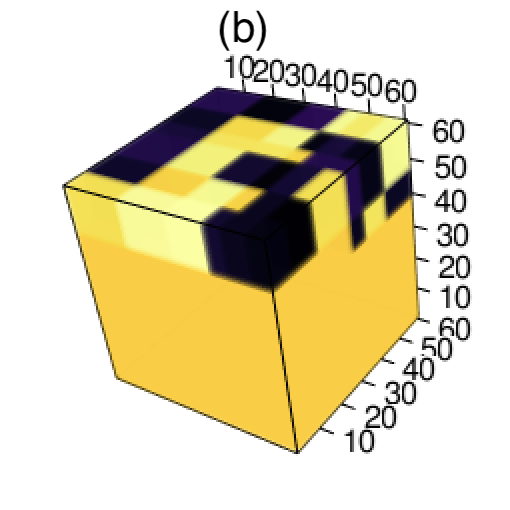
\includegraphics[scale=0.5]{figures/figure2/truth.png}
	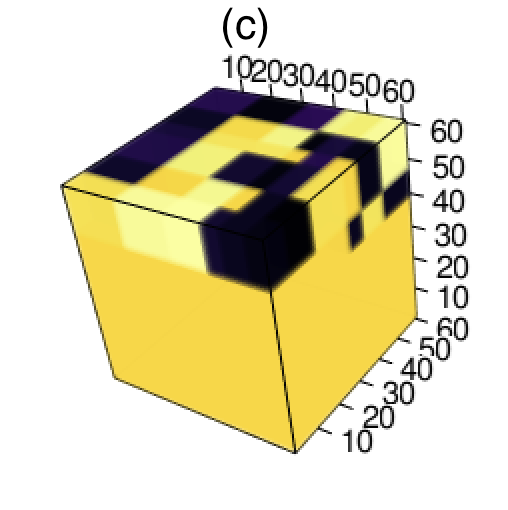
\includegraphics[scale=0.5]{figures/figure2/output.png}
	\caption{(a): 60*60*60 sparse tensor; (b) true underlying means; (c) mean signal estimated by our approach with estimated number of clusters and estimated $\lambda$.}
	\label{fig2}
\end{figure}
\subsection{Notation}
We use $\tT$, $\tX$, and $\tE$ to represent input, signal, and noise tensors, respectively. For any set $J$, $|J|$ denotes its cardinality. $[n]$ represents the set $\{1,2,\ldots,n\}$. $\mx\otimes \my$ is the Kronecker product of two vectors. 
Papers to be submitted to NeurIPS 2018 must be prepared according to the
instructions presented here. Papers may only be up to eight pages long,
including figures. Additional pages \emph{containing only acknowledgments and/or
  cited references} are allowed. Papers that exceed eight pages of content
(ignoring references) will not be reviewed, or in any other way considered for
presentation at the conference.

The margins in 2018 are the same as since 2007, which allow for $\sim$$15\%$
more words in the paper compared to earlier years.

Authors are required to use the NeurIPS \LaTeX{} style files obtainable at the
NeurIPS website as indicated below. Please make sure you use the current files
and not previous versions. Tweaking the style files may be grounds for
rejection.

\subsection{Problem formulation}
In 

\begin{center}
  \url{http://www.neurips.cc/}
\end{center}
The file \verb+neurips_2018.pdf+ contains these instructions and illustrates the
various formatting requirements your NeurIPS paper must satisfy.

The only supported style file for NeurIPS 2018 is \verb+neurips_2018.sty+,
rewritten for \LaTeXe{}.  \textbf{Previous style files for \LaTeX{} 2.09,
  Microsoft Word, and RTF are no longer supported!}

The \LaTeX{} style file contains three optional arguments: \verb+final+, which
creates a camera-ready copy, \verb+preprint+, which creates a preprint for
submission to, e.g., arXiv, and \verb+nonatbib+, which will not load the
\verb+natbib+ package for you in case of package clash.

\paragraph{New preprint option for 2018}
If you wish to post a preprint of your work online, e.g., on arXiv, using the
NeurIPS style, please use the \verb+preprint+ option. This will create a
nonanonymized version of your work with the text ``Preprint. Work in progress.''
in the footer. This version may be distributed as you see fit. Please \textbf{do
  not} use the \verb+final+ option, which should \textbf{only} be used for
papers accepted to NeurIPS.

At submission time, please omit the \verb+final+ and \verb+preprint+
options. This will anonymize your submission and add line numbers to aid
review. Please do \emph{not} refer to these line numbers in your paper as they
will be removed during generation of camera-ready copies.

The file \verb+neurips_2018.tex+ may be used as a ``shell'' for writing your
paper. All you have to do is replace the author, title, abstract, and text of
the paper with your own.

The formatting instructions contained in these style files are summarized in
Sections \ref{gen_inst}, \ref{headings}, and \ref{others} below.

\section{General formatting instructions}
\label{gen_inst}

The text must be confined within a rectangle 5.5~inches (33~picas) wide and
9~inches (54~picas) long. The left margin is 1.5~inch (9~picas).  Use 10~point
type with a vertical spacing (leading) of 11~points.  Times New Roman is the
preferred typeface throughout, and will be selected for you by default.
Paragraphs are separated by \nicefrac{1}{2}~line space (5.5 points), with no
indentation.

The paper title should be 17~point, initial caps/lower case, bold, centered
between two horizontal rules. The top rule should be 4~points thick and the
bottom rule should be 1~point thick. Allow \nicefrac{1}{4}~inch space above and
below the title to rules. All pages should start at 1~inch (6~picas) from the
top of the page.

For the final version, authors' names are set in boldface, and each name is
centered above the corresponding address. The lead author's name is to be listed
first (left-most), and the co-authors' names (if different address) are set to
follow. If there is only one co-author, list both author and co-author side by
side.

Please pay special attention to the instructions in Section \ref{others}
regarding figures, tables, acknowledgments, and references.

\section{Headings: first level}
\label{headings}

All headings should be lower case (except for first word and proper nouns),
flush left, and bold.

First-level headings should be in 12-point type.

\subsection{Headings: second level}

Second-level headings should be in 10-point type.

\subsubsection{Headings: third level}

Third-level headings should be in 10-point type.

\paragraph{Paragraphs}

There is also a \verb+\paragraph+ command available, which sets the heading in
bold, flush left, and inline with the text, with the heading followed by 1\,em
of space.
\section{Tuning Paraneter Selection}
There are four tuning parameters in our tensor clustering proposal: 
\begin{itemize}
	\item the number of clusters in each modes: K (mode 1), R (model 2), L (mode 3);
	\item the penalty coefficient $\lambda$.
\end{itemize}
\subsection{Selection of K, R, L}
We use BIC to select the best K, R, L here. Given a range of K, R, L, we use our former approach to do tensor clustering for all combinations of K, R, L and calculate the BIC for each of them separately using the formula:
\begin{equation*}
	BIC = npq\times log(RSS)+(q+c)log(npq)
\end{equation*}
Here n, p, q denote the dimension of the data in each mode; q is the number of clusters have non-zero means; c denotes the degrees of freedom while doint the clustering.\par 
 Because in non-sparse case, there may be many reasonable K, R, L, we choose the K, R, L which is the smallest among all K, R, L whose BIC is the smallest. The results are shown as Table \ref{t2}. 
\subsection{Selection of $\lambda$}
We use BIC to select the $\lambda$, too. After estimating the K, R, L, we use the estimated K, R, L to do tensor clustering. First we choose a reasonable range for $\lambda$ according to the following theorem:
\begin{theorem}
	Let $\mathbf{Y} \in \mathbb{R}^n$ be a response vector and $\mathbf{X} \in \mathbb{R}^{n\times p}$ the design matrix. Assume the response vector $\mathbf{Y}$ is mean-centered, i.e., $\sum_iY_i=0$. Suppose that $\mathbf{X}$ is an orthogonal design matrix with $X^TX=diag(n_1,...,n_p)$. Define the ordinary least-square estimate $\hat{\bm{\beta}}_{ols} = (\hat{\beta}_{ols,1},...,\hat{\beta}^T_{ols,p})^T$. Consider the following constrained optimization: 
	\begin{equation*}
		\bm{
		\hat{\beta}} = argmin\{\frac{1}{2}||\mathbf{Y}-\mathbf{X}\bm{\beta}||^2_2+\lambda pen(\bm{\beta})\}
	\end{equation*}
	1. Case 1: L-0 penalization. $pen(\bm{\beta}) = ||\bm{\beta}||_0$:\\
	 Under the change of tuning parameter $\lambda' := f(\lambda)=\sqrt{2\lambda}$  such that $\bm{\hat{\beta}} = (\hat{\beta}_1,..., \hat{\beta}_p)^T$ has a closed-form solution:
	\begin{equation*}
		\hat{\beta}_i = \hat{\beta}_{ols,i}\mathbb{I}_{|\hat{\beta}_{ols,i}|>\frac{\lambda'}{\sqrt{n_i}}}\ for\ all\ i=1,...,p
	\end{equation*}
	2. Case 2: L-1 penalization. $pen(\bm{\beta})= ||\bm{\beta}||_1$:\\
	$\bm{\hat{\beta}} = (\hat{\beta}_1,..., \hat{\beta}_p)^T$ has a closed-form solution:
	\begin{equation*}
		\hat{\beta}_i = sign(\hat{\beta_{ols,i}})(|\hat{\beta_{ols,i}}|-\frac{\lambda}{n_i})_+\ for\ all\ i=1,2,...,p
	\end{equation*}
	
\end{theorem}
Next, we do the tensor clustering for all $\lambda$ in the selected range of $\lambda$ and calculate the BIC. Finally we choose the smallest $\lambda$ with smallest BIC. The performance can be evaluated according to the $\bar{\lambda}$ in Table \ref{t4}.
\section{Simulation and Evaluation}
Given the approach of clustering in the former section, we evaluate the performance of it under different conditions: 
\begin{itemize}
	\item given a non-sparse tensor and true cluster numbers of each mode, estimate the underlying mean signal;
	\item given a non-sparse tensor, estimate the cluster numbers of different modes;
	\item given a non-sparse tensor, estimate the underlying mean signal;
	\item given a sparse tensor, choose a appropriate $\lambda$, estimate the cluster numvers of different modes and estimate the underlying mean signal.
\end{itemize}
Here are the statistics we would use to evaluate the performance in different cases:
\begin{itemize}
	\item CER(clustering error rate): the adjusted rand index between two paritions. This statistic measure the agreement between the true partition and estimated partition of the data tensor. In this case, we have three kinds of CER in total: CER of mode 1, CER of mode 2 and CER of mode 3. In non-sparse case, we use CER to evaluate the performance;
	\item Total Incorrect Rate (eg. Table \ref{t4}): the proportion of misjudgement while determining whether the mean signal is zero. We use this in sparse case. Because when the data tensor is sparse, then different clusters can have the same mean: 0. In this case, we can have multiple reasonable partitions of the modes. Thus, CER is inapplicable at this time;
	\item Correct Zero Rate: the proportion of zero elements are correctly identified in the underlying mean tensor;
	\item Correct One Rate: the proportion of non-zero elements are correctly identified in the underlying mean tensor.
\end{itemize}
Here we give a brief elaboration on how to generate the data. As for non-sparse tensor, given the cluster numbers K, R, L and the size of the tensor n*p*q, we assign the labels to each modes randomly. Next we randomly select the mean signal of clusters from Unif(-3,3) and add noise which comes from normal distribution with given standard deviation. Then we get the non-sparse tensor. As for sparse tensor, we randomly assign 0 to the mean of some  clusters with given sparsity rate (the proportion of 0 elements) and then follow the same steps.
\subsection{Simulation 1: clustering results with true cluster numers in each mode (non-sparse tensor)}
We generate 50 non-sparse tensors with the same noise, size and cluster numbers each time. Here we choose $K=3$, $R=5$, $L=4$ specifically. We use our approach (Algorithm \ref{alg:B}) to do the clustering with given K,R,L and the result is shown as Table \ref{t1}.\par 
In both data size: 40*40*40 and 50*50*50, the CER on all modes are 0 when the noise is 0 and 5. As the noise goes up, the CER is increased. Furthermore, the CER becomes smaller as the data size become larger.
\begin{table}
	\centering
	\begin{tabular}{|c|c|c|c|c|c|c|}
		\hline
		n&p&q&noise&cer(mode 1)&cer(mode 2)&cer(mode3)\\ \hline
		40&40&40&0&0(0)&0(0)&0(0) \\
		40&40&40&5&0(0)&0(0)&0(0) \\
		40&40&40&10&0.0021(0.0145)&0.0231(0.0393)&0.0106 (0.0368)\\
		40&40&40&15&0.1983(0.1532)&0.1768(0.0834)&0.1906(0.1138) \\
		50&50&50&0&0(0)&0(0)&0(0) \\
		50&50&50&5&0(0)&0(0)&0(0) \\
		50&50&50&10&0(0)&0.0043(0.0181)&0.0024(0.0173) \\
		50&50&50&15&0.0133(0.0441)&0.0485(0.0514)&0.0258(0.0578) \\
		\hline
	\end{tabular}
	\caption{Results for Simulation 1 over 50 simulated data sets (k=3, r=5, l=4)}
	\label{t1}
\end{table}
\subsection{Simulation 2: estimation on cluster numbers (non-sparse tensor)}
We generate 50 non-sparse tensors with the same noise, size and cluster numbers in each case in Table \ref{t2}. As expected, the overall accuracy goes down as the noise increased, and goes up as the data size increased. 
Finally, we only evaluate the performance of estimation on cluster numbers on non-sparse tensor, because in sparse case, the reasonable cluster numbers may not be unique.
\begin{table}
	\centering
	\resizebox{\textwidth}{20mm}{
	\begin{tabular}{|c|c|c|c|c|c|c|c|c|c|c|}
		\hline
		n&p&q&K&R&L&noise&overall accuracy&estimated K&estimated R&estimated L\\ \hline
		40&40&40&3&5&4&1&0.98&3(0)&5(0)&4.02(0.02)\\
		40&40&40&3&5&4&4&1&3(0)&5(0)&4(0)\\
		40&40&40&3&5&4&8&0.7&3 (0)&4.72(0.0641427)&3.98(0.02)\\
		40&40&40&3&4&2&1&1&3(0)&4(0)&2(0)\\
		40&40&40&3&4&2&4&1&3(0)&4(0)&2(0)\\
		40&40&40&3&4&2&8&0.88&3 (0)&3.88(0.0464)&2 (0)\\
		50&50&50&3&4&2&1&1&3(0)&4(0)&2(0)\\
		50&50&50&3&4&2&4&1&3(0)&4(0)&2(0)\\
		50&50&50&3&4&2&8&0.98&3 (0)&3.98(0.02)&2 (0)\\
		\hline
	\end{tabular}}
	\caption{Results for Simulation 2 over 50 simulated data sets}
	\label{t2}
\end{table}
\subsection{Simulation 3: clustering results without given true cluster numbers in each mode (non-sparse tensor) }
In this simulation, the true cluster numbers are not given, so we estimate them first and then use the estimated true cluster numbers to estimate the parition of clusters as well as underlying mean signals. We set the true cluster numbers to be $K=3, R=5, L=4$, and the results are shown in Table \ref{t3}.
\begin{table}
	\centering
	\begin{tabular}{|c|c|c|c|c|c|c|}
		\hline
		n&p&q&noise&cer(mode 1)&cer(mode 2)&cer(mode3)\\ \hline
		40&40&40&1&0(0)&0(0)&0(0) \\
		40&40&40&4&0(0)&0(0)&0(0) \\
		40&40&40&8&0(0)&0.013(0.0226)&0.0106 (0.0368)\\
		50&50&50&1&0(0)&0(0)&0(0) \\
		50&50&50&4&0(0)&0(0)&0(0) \\
		50&50&50&8&0(0)&0.0014(0.0102)&0.0024(0.0173) \\
		\hline
	\end{tabular}
	\caption{Results for Simulation 3 over 50 simulated data sets (K=3, R=5, L=4)}
	\label{t3}
\end{table}
\subsection{Simulation 4: clustering results without given true cluster numbers in each mode (sparse tensor)}
We also test the performace of our approach under different $\lambda$ when the data is sparse. The $\bar{\lambda}$ in Table \ref{t4} is the mean $\lambda$ we choose across 50 simulations on the same sparsity rate. According to Table \ref{t4}, the correct zero rate is increased with the increment on $\lambda$ while the correct one rate is exactly the opposite. As for the $\lambda$ we choose, it shows that the total incorrect rate all are lower than 0.06 here, indicating approximately 94\% accuracy among the three cases.
\begin{table}
	\centering
	\resizebox{\textwidth}{25mm}{
	\begin{tabular}{|c|c|c|c|c|c|c|}
		\hline
		sparsity rate&error&method&estimated sparsity Rate&Correct Zero Rate&Correct One Rate&Total Incorrect Rate  \\ \hline
		0.5&1&$\lambda=0$&0 ( 0 ) &0 ( 0 )&1 ( 0 )&0.4925 ( 0.0676 )\\
		0.5&1&$\lambda=5$&0.5235 ( 0.0661) & 1 ( 0 )& 0.9396 ( 0.0499 )&0.0310 ( 0.0269 )\\
		0.5&1&$\lambda=10$&0.5489 ( 0.0655 ) & 1 ( 0 )&0.8890( 0.0540)&0.0564 ( 0.0297 )\\
		0.5&1&$\lambda=15$&0.5706 ( 0.0703 )&1 ( 0 )& 0.8455( 0.0715 )& 0.0781 ( 0.0386 )\\
		0.5&1&$\bar{\lambda}=4.0825$&0.5201 ( 0.0648 )&1 ( 0 )&0.9467 ( 0.0489 ) &0.0276 ( 0.0266)\\
		0.5&3&$\lambda=0$&0 ( 0 ) &0 ( 0 )&1 ( 0 )&0.4925 ( 0.0676 )\\
		0.5&3&$\lambda=5$& 0.4556 ( 0.0671 ) & 0.8647 ( 0.0828 )&0.9404 ( 0.0512 )& 0.0975 ( 0.0507 )\\
		0.5&3&$\lambda=10$&0.5475 ( 0.0654 )&0.9997 ( 0.0024 )&0.8914 ( 0.0548 )&0.0554 ( 0.03)\\
		0.5&3&$\lambda=15$&0.5717 ( 0.0672 )&1 ( 0 )&0.844 ( 0.0691 )& 0.0792 ( 0.0388 )\\
		0.5&3&$\bar{\lambda}=10.71244$&0.5513 ( 0.0661 )&1 ( 0 )&0.8843 ( 0.0573 ) &0.0588 ( 0.0311 )\\
		0.8&1&$\lambda=0$&0 ( 0 ) &0 ( 0 )&1 ( 0 )&0.7971 ( 0.0541 )\\
		0.8&1&$\lambda=5$&0.807 ( 0.0558 ) & 1 ( 0 )& 0.9477 ( 0.0658 )&0.0099 ( 0.0132 )\\
		0.8&1&$\lambda=10$&0.8148 ( 0.0573 )& 1 ( 0 )&0.9057 ( 0.0925 )&0.0177 ( 0.0182 )\\
		0.8&1&$\lambda=15$&0.8249 ( 0.0587 )&1 ( 0 )& 0.8537 ( 0.1164 )&0.0278 ( 0.0232 )\\
		0.8&1&$\bar{\lambda}=3.527265$&0.8034 ( 0.056 )&0.9978 ( 0.0105 )&0.9566 ( 0.0625 )&0.0099 ( 0.0139 )\\
		\hline
	\end{tabular}}
	\caption{Results for Simulation 4 over 50 simulated data sets (n=40, p=40, q=40,  K=3, R=5, L=4)}
	\label{t4}
\end{table}

\subsection{Citations within the text}

The \verb+natbib+ package will be loaded for you by default.  Citations may be
author/year or numeric, as long as you maintain internal consistency.  As to the
format of the references themselves, any style is acceptable as long as it is
used consistently.

The documentation for \verb+natbib+ may be found at
\begin{center}
  \url{http://mirrors.ctan.org/macros/latex/contrib/natbib/natnotes.pdf}
\end{center}
Of note is the command \verb+\citet+, which produces citations appropriate for
use in inline text.  For example,
\begin{verbatim}
   \citet{hasselmo} investigated\dots
\end{verbatim}
produces
\begin{quote}
  Hasselmo, et al.\ (1995) investigated\dots
\end{quote}

If you wish to load the \verb+natbib+ package with options, you may add the
following before loading the \verb+neurips_2018+ package:
\begin{verbatim}
   \PassOptionsToPackage{options}{natbib}
\end{verbatim}

If \verb+natbib+ clashes with another package you load, you can add the optional
argument \verb+nonatbib+ when loading the style file:
\begin{verbatim}
   \usepackage[nonatbib]{neurips_2018}
\end{verbatim}

As submission is double blind, refer to your own published work in the third
person. That is, use ``In the previous work of Jones et al.\ [4],'' not ``In our
previous work [4].'' If you cite your other papers that are not widely available
(e.g., a journal paper under review), use anonymous author names in the
citation, e.g., an author of the form ``A.\ Anonymous.''

\subsection{Footnotes}

Footnotes should be used sparingly.  If you do require a footnote, indicate
footnotes with a number\footnote{Sample of the first footnote.} in the
text. Place the footnotes at the bottom of the page on which they appear.
Precede the footnote with a horizontal rule of 2~inches (12~picas).

Note that footnotes are properly typeset \emph{after} punctuation
marks.\footnote{As in this example.}

\subsection{Figures}

\begin{figure}
  \centering
  \fbox{\rule[-.5cm]{0cm}{4cm} \rule[-.5cm]{4cm}{0cm}}
  \caption{Sample figure caption.}
\end{figure}

All artwork must be neat, clean, and legible. Lines should be dark enough for
purposes of reproduction. The figure number and caption always appear after the
figure. Place one line space before the figure caption and one line space after
the figure. The figure caption should be lower case (except for first word and
proper nouns); figures are numbered consecutively.

You may use color figures.  However, it is best for the figure captions and the
paper body to be legible if the paper is printed in either black/white or in
color.

\subsection{Tables}

All tables must be centered, neat, clean and legible.  The table number and
title always appear before the table.  See Table~\ref{sample-table}.

Place one line space before the table title, one line space after the
table title, and one line space after the table. The table title must
be lower case (except for first word and proper nouns); tables are
numbered consecutively.

Note that publication-quality tables \emph{do not contain vertical rules.} We
strongly suggest the use of the \verb+booktabs+ package, which allows for
typesetting high-quality, professional tables:
\begin{center}
  \url{https://www.ctan.org/pkg/booktabs}
\end{center}
This package was used to typeset Table~\ref{sample-table}.

\begin{table}
  \caption{Sample table title}
  \label{sample-table}
  \centering
  \begin{tabular}{lll}
    \toprule
    \multicolumn{2}{c}{Part}                   \\
    \cmidrule(r){1-2}
    Name     & Description     & Size ($\mu$m) \\
    \midrule
    Dendrite & Input terminal  & $\sim$100     \\
    Axon     & Output terminal & $\sim$10      \\
    Soma     & Cell body       & up to $10^6$  \\
    \bottomrule
  \end{tabular}
\end{table}

\section{Final instructions}

Do not change any aspects of the formatting parameters in the style files.  In
particular, do not modify the width or length of the rectangle the text should
fit into, and do not change font sizes (except perhaps in the
\textbf{References} section; see below). Please note that pages should be
numbered.

\section{Preparing PDF files}

Please prepare submission files with paper size ``US Letter,'' and not, for
example, ``A4.''

Fonts were the main cause of problems in the past years. Your PDF file must only
contain Type 1 or Embedded TrueType fonts. Here are a few instructions to
achieve this.

\begin{itemize}

\item You should directly generate PDF files using \verb+pdflatex+.

\item You can check which fonts a PDF files uses.  In Acrobat Reader, select the
  menu Files$>$Document Properties$>$Fonts and select Show All Fonts. You can
  also use the program \verb+pdffonts+ which comes with \verb+xpdf+ and is
  available out-of-the-box on most Linux machines.

\item The IEEE has recommendations for generating PDF files whose fonts are also
  acceptable for NeurIPS. Please see
  \url{http://www.emfield.org/icuwb2010/downloads/IEEE-PDF-SpecV32.pdf}

\item \verb+xfig+ "patterned" shapes are implemented with bitmap fonts.  Use
  "solid" shapes instead.

\item The \verb+\bbold+ package almost always uses bitmap fonts.  You should use
  the equivalent AMS Fonts:
\begin{verbatim}
   \usepackage{amsfonts}
\end{verbatim}
followed by, e.g., \verb+\mathbb{R}+, \verb+\mathbb{N}+, or \verb+\mathbb{C}+
for $\mathbb{R}$, $\mathbb{N}$ or $\mathbb{C}$.  You can also use the following
workaround for reals, natural and complex:
\begin{verbatim}
   \newcommand{\RR}{I\!\!R} %real numbers
   \newcommand{\Nat}{I\!\!N} %natural numbers
   \newcommand{\CC}{I\!\!\!\!C} %complex numbers
\end{verbatim}
Note that \verb+amsfonts+ is automatically loaded by the \verb+amssymb+ package.

\end{itemize}

If your file contains type 3 fonts or non embedded TrueType fonts, we will ask
you to fix it.

\subsection{Margins in \LaTeX{}}

Most of the margin problems come from figures positioned by hand using
\verb+\special+ or other commands. We suggest using the command
\verb+\includegraphics+ from the \verb+graphicx+ package. Always specify the
figure width as a multiple of the line width as in the example below:
\begin{verbatim}
   \usepackage[pdftex]{graphicx} ...
   \includegraphics[width=0.8\linewidth]{myfile.pdf}
\end{verbatim}
See Section 4.4 in the graphics bundle documentation
(\url{http://mirrors.ctan.org/macros/latex/required/graphics/grfguide.pdf})

A number of width problems arise when \LaTeX{} cannot properly hyphenate a
line. Please give LaTeX hyphenation hints using the \verb+\-+ command when
necessary.

\subsubsection*{Acknowledgments}

Use unnumbered third level headings for the acknowledgments. All acknowledgments
go at the end of the paper. Do not include acknowledgments in the anonymized
submission, only in the final paper.

\section*{References}

References follow the acknowledgments. Use unnumbered first-level heading for
the references. Any choice of citation style is acceptable as long as you are
consistent. It is permissible to reduce the font size to \verb+small+ (9 point)
when listing the references. {\bf Remember that you can use more than eight
  pages as long as the additional pages contain \emph{only} cited references.}
\medskip

\small

[1] Alexander, J.A.\ \& Mozer, M.C.\ (1995) Template-based algorithms for
connectionist rule extraction. In G.\ Tesauro, D.S.\ Touretzky and T.K.\ Leen
(eds.), {\it Advances in Neural Information Processing Systems 7},
pp.\ 609--616. Cambridge, MA: MIT Press.

[2] Bower, J.M.\ \& Beeman, D.\ (1995) {\it The Book of GENESIS: Exploring
  Realistic Neural Models with the GEneral NEural SImulation System.}  New York:
TELOS/Springer--Verlag.

[3] Hasselmo, M.E., Schnell, E.\ \& Barkai, E.\ (1995) Dynamics of learning and
recall at excitatory recurrent synapses and cholinergic modulation in rat
hippocampal region CA3. {\it Journal of Neuroscience} {\bf 15}(7):5249-5262.

\begin{appendices}
	\section{Proof of Theorems}
	\begin{proof}
		The thing we want to minimize is
		\begin{equation*}
		L=\frac{1}{2}||\mathbf{Y-X}\bm{\beta}||^2_2+\lambda||\bm{\beta}_0||=\frac{1}{2}(\mathbf{Y-X}\bm{\beta})^T(\mathbf{Y-X}\bm{\beta})+\lambda ||\bm{\beta}||_0=L_1+L_2
		\end{equation*} 
		where $L_1=\frac{1}{2}(\mathbf{Y-X}\bm{\beta})^T(\mathbf{Y-X}\bm{\beta})$, $L_2=\lambda ||\bm{\beta}||_0$. 
	
	\textbf{Case 1:}\par 
	 Here we view the optimization problem as a case in linear regression. 
	The $L_1$ is exactly the $RSS/2$ in this case. So we compare the increment of $L_1$  when $L_2$ takes different values. We denote $z$ as the number of  non-zero elements in $\bm{\beta}$.\\
	(1) Consider the case we have no constraint on $z$. Thus we only have to minimize $L_1$. By the knowledge of linear regression, we know the unique minimizer is $\bm{\hat{\beta}_{ols}}=\mathbf{(X^TX)^{-1}XY}$. Assume there are $m$ zero elements in $\bm{\hat{\beta}_{ols}}$ where $0\leq m \leq p$ \\
	(2) Consider the case we have constraint on $z$: $z = i$, where $i=0,1,2,...,m$. Obviously, among these cases the $L$ can be minimized if and only if $i=m$. So, $z=m$ and $\bm{\hat{\beta}}=\bm{\hat{\beta}_{ols}}$ is the minimizer of $L$ when $0\leq z\leq m$.
	(3) Consider the case that we have constraint on $x$: $z=m+1$. Then we have to take one more non-zero element in $\bm{\beta}$ to be zero. Suppose we take $\hat{\beta}_l \neq 0$ to be 0. Then we obtain 
	\begin{equation*}
		2L_1 -SSE(\beta_1,...,\beta_{l-1},\beta_{l+1},...,\beta_p)=SSR(\beta_l)
	\end{equation*}
	by the columns in $\mathbf{X}$ are orthogonal to each other. Additionally,
	\begin{equation*}
		SSR(\beta_l) = \mathbf{Y}^T(\mathbf{H-H_l})\mathbf{Y} 
	\end{equation*}
	where $\mathbf{H=X(X^TX)^{-1}X}=\sum_{i=1}^p\frac{1}{n_i}\mathbf{x_{(i)}x_{(i)}^T}$, $\mathbf{H_l} = \sum_{i\neq j}\mathbf{x_{(i)}x_{(i)}^T}$, $\hat{\beta}_l = \frac{1}{n_l}\mathbf{x_{l}Y}$. Thus, we can simplify the second equation as:
	\begin{equation*}
		SSR(\beta_l) = n_l\hat{\beta}_l^2
	\end{equation*}
	Thus, by taking $\hat{\beta}_l$ as 0, there is $\frac{n_l\hat{\beta}_l^2}{2}$ increment on $L_1$, $\lambda$ decrement on $L_2$. Obviously, if the increment of $L_1$ is larger than the decrement $L_2$, we should not take $\hat{\beta_l}$ as 0; conversely, if the increment of $L_1$ is less than the decrement of $L_2$, taking $\hat{\beta_l}$ as 0 can lessen the L.\\
	(4) As we discussed, if there is still at least one element in $\bm{\beta_k}$ that satisfies that $\frac{n_k\hat{\beta}_k^2}{2}\leq\lambda$, we can keep reducing $L$ by taking $\bm{\beta_k}$ as 0 until all remain non-zero elements in $\hat{\beta}$ do not satisfy $\frac{n_k\hat{\beta}_k^2}{2}\leq\lambda$. Then we can minimize $L$.\par 
	Over all, the $\bm{\beta}$ that minimized $L$ is:
	\begin{equation*}
			\hat{\beta}_i = \hat{\beta}_{ols,i}\mathbb{I}_{|\hat{\beta}_{ols,i}|>\frac{\lambda'}{\sqrt{n_i}}}\ for\ all\ i=1,...,p
	\end{equation*}
	
\textbf{Case 2:}\par
Here we use the properties of subderivative. Taking subderivative of $L$, we obtain
	
\begin{equation*}
\frac{\partial L}{\partial \beta_j} = 
\begin{cases}
\{n_j\beta_j-\mathbf{x_{(j)}^TY}+\lambda\} &\mbox{if $\beta_j>0$}\\
 [n_j\beta_j-\mathbf{x_{(j)}^TY}-\lambda, n_j\beta_j-\mathbf{x_{(j)}^TY}+\lambda]&\mbox{if $\beta_j=0$}\\
\{n_j\beta_j-\mathbf{x_{(j)}^TY}-\lambda\} &\mbox{if $\beta_j<0$}\\
\end{cases}
\end{equation*}
Because $\beta_j$ minimize $L$ if and only if $0 \in \frac{\partial L}{\partial \beta_j}$ and  $\mathbf{X}$ is orthogonal, we get:
\begin{equation*}
\hat{\beta_j} = 
\begin{cases}
\frac{\mathbf{x_{(j)}^TY}+\lambda}{n_j}&\mbox{if $\hat{\beta_j}<0$}\\
0 &\mbox{if $\hat{\beta_j}=0$}\\
\frac{\mathbf{x_{(j)}^TY}-\lambda}{n_j}&\mbox{if $\hat{\beta_j}>0$}\\
\end{cases}
\end{equation*}
Here, $\bm{\hat{\beta}}_{ols} = \mathbf{(X^TX)^{-1}X^TY} = diag(1/n_1, ..., 1/n_p)X^TY$, so $\hat{\beta}_{ols,j}=\frac{\mathbf{x_{(j)}^TY}}{n_j}$. Then the solution of $\hat{\beta_j}$ can be simplified as:
\begin{equation*}
	\hat{\beta}_i = sign(\hat{\beta_{ols,i}})(|\hat{\beta_{ols,i}}|-\frac{\lambda}{n_i})_+\ for\ all\ i=1,2,...,p
\end{equation*}
\end{proof}
	\section{Algorithm}
	\begin{algorithm}
		\caption{Block Localization}
		\label{alg:B}
		\begin{algorithmic}
			\STATE {Initialize $C_1,...,C_K$,$D_1,...,D_R$ and $E_1,...,E_L$ by performing one-way k-means clustering on the columns and on the rows of the data matrix $X$.}
			\REPEAT 
			\STATE (a) Holding $C_1,...,C_K$,$D_1,...,D_R$ and $E_1,...,E_L$ fixed, solve (1) with respect to $\mathbf{\mu}$ using LASSO regression.
			\STATE (b) Holding  $\mathbf{\mu}$, $D_1,...,D_R$ and $E_1,...,E_L$ fixed, solve (1) with respect to $C_1,...,C_K$, by assigning the $i$th observation to the row cluster for which $\sum_{r=1}^R\sum_{l=1}^L\sum_{j\in D_r}\sum_{m\in E_l}(X_{ijm}-\mu_{krl})^2$ is smallest.
			\STATE (c) repeat (a).
			\STATE (d) Holding  $\mathbf{\mu}$, $C_1,...,C_K$ and $E_1,...,E_L$ fixed, solve (1) with respect to $D_1,...,D_R$, by assigning the $i$th observation to the column cluster for which $\sum_{k=1}^K\sum_{l=1}^L\sum_{i\in C_k}\sum_{m\in E_l}(X_{ijm}-\mu_{krl})^2$ is smallest.
			\STATE (e) repeat (a).
			\STATE (f) Holding  $\mathbf{\mu}$, $C_1,...,C_K$ and $D_1,...,D_R$ fixed, solve (1) with respect to $E_1,...,E_L$, by assigning the $i$th observation to the cluster of the third dimension for which $\sum_{k=1}^K\sum_{r=1}^R\sum_{i\in C_k}\sum_{j\in D_r}(X_{ijm}-\mu_{krl})^2$ is smallest.
			\UNTIL{Convergence} 
		\end{algorithmic}
	\end{algorithm}

\end{appendices}
\end{document}
